\PassOptionsToPackage{unicode=true}{hyperref} % options for packages loaded elsewhere
\PassOptionsToPackage{hyphens}{url}
%
\documentclass[]{article}
\usepackage{lmodern}
\usepackage{amssymb,amsmath}
\usepackage{ifxetex,ifluatex}
\usepackage{fixltx2e} % provides \textsubscript
\ifnum 0\ifxetex 1\fi\ifluatex 1\fi=0 % if pdftex
  \usepackage[T1]{fontenc}
  \usepackage[utf8]{inputenc}
  \usepackage{textcomp} % provides euro and other symbols
\else % if luatex or xelatex
  \usepackage{unicode-math}
  \defaultfontfeatures{Ligatures=TeX,Scale=MatchLowercase}
\fi
% use upquote if available, for straight quotes in verbatim environments
\IfFileExists{upquote.sty}{\usepackage{upquote}}{}
% use microtype if available
\IfFileExists{microtype.sty}{%
\usepackage[]{microtype}
\UseMicrotypeSet[protrusion]{basicmath} % disable protrusion for tt fonts
}{}
\IfFileExists{parskip.sty}{%
\usepackage{parskip}
}{% else
\setlength{\parindent}{0pt}
\setlength{\parskip}{6pt plus 2pt minus 1pt}
}
\usepackage{hyperref}
\hypersetup{
            pdftitle={Noura Analysis of RNAseq studies},
            pdfauthor={Dave Bridges, Noura El Habbal},
            pdfborder={0 0 0},
            breaklinks=true}
\urlstyle{same}  % don't use monospace font for urls
\usepackage[margin=1in]{geometry}
\usepackage{color}
\usepackage{fancyvrb}
\newcommand{\VerbBar}{|}
\newcommand{\VERB}{\Verb[commandchars=\\\{\}]}
\DefineVerbatimEnvironment{Highlighting}{Verbatim}{commandchars=\\\{\}}
% Add ',fontsize=\small' for more characters per line
\usepackage{framed}
\definecolor{shadecolor}{RGB}{248,248,248}
\newenvironment{Shaded}{\begin{snugshade}}{\end{snugshade}}
\newcommand{\AlertTok}[1]{\textcolor[rgb]{0.94,0.16,0.16}{#1}}
\newcommand{\AnnotationTok}[1]{\textcolor[rgb]{0.56,0.35,0.01}{\textbf{\textit{#1}}}}
\newcommand{\AttributeTok}[1]{\textcolor[rgb]{0.77,0.63,0.00}{#1}}
\newcommand{\BaseNTok}[1]{\textcolor[rgb]{0.00,0.00,0.81}{#1}}
\newcommand{\BuiltInTok}[1]{#1}
\newcommand{\CharTok}[1]{\textcolor[rgb]{0.31,0.60,0.02}{#1}}
\newcommand{\CommentTok}[1]{\textcolor[rgb]{0.56,0.35,0.01}{\textit{#1}}}
\newcommand{\CommentVarTok}[1]{\textcolor[rgb]{0.56,0.35,0.01}{\textbf{\textit{#1}}}}
\newcommand{\ConstantTok}[1]{\textcolor[rgb]{0.00,0.00,0.00}{#1}}
\newcommand{\ControlFlowTok}[1]{\textcolor[rgb]{0.13,0.29,0.53}{\textbf{#1}}}
\newcommand{\DataTypeTok}[1]{\textcolor[rgb]{0.13,0.29,0.53}{#1}}
\newcommand{\DecValTok}[1]{\textcolor[rgb]{0.00,0.00,0.81}{#1}}
\newcommand{\DocumentationTok}[1]{\textcolor[rgb]{0.56,0.35,0.01}{\textbf{\textit{#1}}}}
\newcommand{\ErrorTok}[1]{\textcolor[rgb]{0.64,0.00,0.00}{\textbf{#1}}}
\newcommand{\ExtensionTok}[1]{#1}
\newcommand{\FloatTok}[1]{\textcolor[rgb]{0.00,0.00,0.81}{#1}}
\newcommand{\FunctionTok}[1]{\textcolor[rgb]{0.00,0.00,0.00}{#1}}
\newcommand{\ImportTok}[1]{#1}
\newcommand{\InformationTok}[1]{\textcolor[rgb]{0.56,0.35,0.01}{\textbf{\textit{#1}}}}
\newcommand{\KeywordTok}[1]{\textcolor[rgb]{0.13,0.29,0.53}{\textbf{#1}}}
\newcommand{\NormalTok}[1]{#1}
\newcommand{\OperatorTok}[1]{\textcolor[rgb]{0.81,0.36,0.00}{\textbf{#1}}}
\newcommand{\OtherTok}[1]{\textcolor[rgb]{0.56,0.35,0.01}{#1}}
\newcommand{\PreprocessorTok}[1]{\textcolor[rgb]{0.56,0.35,0.01}{\textit{#1}}}
\newcommand{\RegionMarkerTok}[1]{#1}
\newcommand{\SpecialCharTok}[1]{\textcolor[rgb]{0.00,0.00,0.00}{#1}}
\newcommand{\SpecialStringTok}[1]{\textcolor[rgb]{0.31,0.60,0.02}{#1}}
\newcommand{\StringTok}[1]{\textcolor[rgb]{0.31,0.60,0.02}{#1}}
\newcommand{\VariableTok}[1]{\textcolor[rgb]{0.00,0.00,0.00}{#1}}
\newcommand{\VerbatimStringTok}[1]{\textcolor[rgb]{0.31,0.60,0.02}{#1}}
\newcommand{\WarningTok}[1]{\textcolor[rgb]{0.56,0.35,0.01}{\textbf{\textit{#1}}}}
\usepackage{graphicx,grffile}
\makeatletter
\def\maxwidth{\ifdim\Gin@nat@width>\linewidth\linewidth\else\Gin@nat@width\fi}
\def\maxheight{\ifdim\Gin@nat@height>\textheight\textheight\else\Gin@nat@height\fi}
\makeatother
% Scale images if necessary, so that they will not overflow the page
% margins by default, and it is still possible to overwrite the defaults
% using explicit options in \includegraphics[width, height, ...]{}
\setkeys{Gin}{width=\maxwidth,height=\maxheight,keepaspectratio}
\setlength{\emergencystretch}{3em}  % prevent overfull lines
\providecommand{\tightlist}{%
  \setlength{\itemsep}{0pt}\setlength{\parskip}{0pt}}
\setcounter{secnumdepth}{5}
% Redefines (sub)paragraphs to behave more like sections
\ifx\paragraph\undefined\else
\let\oldparagraph\paragraph
\renewcommand{\paragraph}[1]{\oldparagraph{#1}\mbox{}}
\fi
\ifx\subparagraph\undefined\else
\let\oldsubparagraph\subparagraph
\renewcommand{\subparagraph}[1]{\oldsubparagraph{#1}\mbox{}}
\fi

% set default figure placement to htbp
\makeatletter
\def\fps@figure{htbp}
\makeatother


\title{Noura Analysis of RNAseq studies}
\author{Dave Bridges, Noura El Habbal}
\date{September 2, 2020}

\begin{document}
\maketitle

{
\setcounter{tocdepth}{2}
\tableofcontents
}
\hypertarget{purpose}{%
\section{Purpose}\label{purpose}}

To analyse aTSC mammary gland RNAseq dataset

\hypertarget{experimental-details}{%
\section{Experimental Details}\label{experimental-details}}

Prior to this analysis, reads were mapped to GRCm38 CDS via Salmon v
1.3.0 with flags \texttt{-\/-gc-bias}, \texttt{-\/-validateMappings} and
\texttt{-l\ A}. These data were saved into the quants folders.

\begin{Shaded}
\begin{Highlighting}[]
\KeywordTok{library}\NormalTok{(tximport) }\CommentTok{#loads the tximport package, needed to bring in the salmon files}
\NormalTok{quant.directories <-}\StringTok{ 'quants'}
\NormalTok{sample.directories <-}\StringTok{ }\KeywordTok{list.dirs}\NormalTok{(quant.directories, }
                                \DataTypeTok{recursive=}\NormalTok{F) }\CommentTok{#identify directories that contain salmon output}
\NormalTok{sample.directories <-}\StringTok{ }\NormalTok{sample.directories[}\KeywordTok{grepl}\NormalTok{(}\StringTok{'NEH'}\NormalTok{, sample.directories)] }\CommentTok{#only noura samples}
\NormalTok{salmon.files <-}\StringTok{ }\KeywordTok{file.path}\NormalTok{(sample.directories,}\StringTok{"quant.sf"}\NormalTok{) }\CommentTok{#locate quant files for each directory}
\NormalTok{salmon.files <-}\StringTok{ }\NormalTok{salmon.files[}\KeywordTok{file.exists}\NormalTok{(salmon.files)]}

\KeywordTok{library}\NormalTok{(}\StringTok{"tximeta"}\NormalTok{)}

\NormalTok{WT <-}\StringTok{ }\KeywordTok{c}\NormalTok{(}\DecValTok{2}\NormalTok{,}\DecValTok{4}\NormalTok{,}\DecValTok{6}\NormalTok{,}\DecValTok{8}\NormalTok{,}\DecValTok{10}\NormalTok{)}
\NormalTok{WT.names <-}\StringTok{ }\KeywordTok{paste}\NormalTok{(}\StringTok{'1415-NEH-'}\NormalTok{,WT, }\DataTypeTok{sep=}\StringTok{""}\NormalTok{)}
\NormalTok{KO <-}\StringTok{ }\KeywordTok{c}\NormalTok{(}\DecValTok{1}\NormalTok{,}\DecValTok{3}\NormalTok{,}\DecValTok{5}\NormalTok{,}\DecValTok{7}\NormalTok{,}\DecValTok{9}\NormalTok{,}\DecValTok{11}\NormalTok{)}
\NormalTok{KO.names <-}\StringTok{ }\KeywordTok{paste}\NormalTok{(}\StringTok{'1415-NEH-'}\NormalTok{,KO, }\DataTypeTok{sep=}\StringTok{""}\NormalTok{)}


\NormalTok{coldata <-}\StringTok{ }\KeywordTok{data.frame}\NormalTok{(}\DataTypeTok{files=}\NormalTok{salmon.files, }
                      \DataTypeTok{stringsAsFactors =}\NormalTok{ F) }\OperatorTok
\StringTok{  }\KeywordTok{separate}\NormalTok{(}\DataTypeTok{col=}\NormalTok{files,}
           \DataTypeTok{sep=}\StringTok{'_'}\NormalTok{,}
           \DataTypeTok{into=}\KeywordTok{c}\NormalTok{(}\StringTok{'Folder'}\NormalTok{,}\StringTok{'names'}\NormalTok{),}
           \DataTypeTok{remove=}\NormalTok{F) }\OperatorTok
\StringTok{  }\KeywordTok{mutate}\NormalTok{(}\DataTypeTok{Genotype=}\KeywordTok{case_when}\NormalTok{(names }\OperatorTok\StringTok{ }\NormalTok{WT.names}\OperatorTok{~}\StringTok{'WT'}\NormalTok{,}
\NormalTok{                            names }\OperatorTok\StringTok{ }\NormalTok{KO.names}\OperatorTok{~}\StringTok{'KO'}\NormalTok{)) }\OperatorTok
\StringTok{  }\KeywordTok{mutate}\NormalTok{(}\DataTypeTok{Genotype =} \KeywordTok{relevel}\NormalTok{(}\KeywordTok{as.factor}\NormalTok{(Genotype), }\DataTypeTok{ref=}\StringTok{"WT"}\NormalTok{))}

\KeywordTok{makeLinkedTxome}\NormalTok{(}\DataTypeTok{indexDir=}\StringTok{'mouse_index'}\NormalTok{,}
                \DataTypeTok{source=}\StringTok{"Ensembl"}\NormalTok{, }\DataTypeTok{organism=}\StringTok{"Mus musculus"}\NormalTok{,}
                \DataTypeTok{release=}\StringTok{"101"}\NormalTok{, }\DataTypeTok{genome=}\StringTok{"GRCm38.101"}\NormalTok{,}
                \DataTypeTok{fasta=}\StringTok{'Mus_musculus.GRCm38.cds.all.fa.gz'}\NormalTok{,}
                \DataTypeTok{gtf=}\StringTok{'Mus_musculus.GRCm38.101.gtf.gz'}\NormalTok{)}

\NormalTok{se <-}\StringTok{ }\KeywordTok{tximeta}\NormalTok{(coldata) }\CommentTok{# looks at all transcripts  and combines them together}
\CommentTok{#se.exons <- addExons(se) #to summarize to gene level data (individual exons, not done yet)}
\NormalTok{gse <-}\StringTok{ }\KeywordTok{summarizeToGene}\NormalTok{(se) }\CommentTok{# the total number of genes 22Kx11 samples}
\end{Highlighting}
\end{Shaded}

These data can be found in
\textbf{/Users/davebrid/Documents/GitHub/TissueSpecificTscKnockouts/RNAseq/Mammary
Gland Adipocyte Tsc1 Knockout} in a set of folders located in quants.
This script was most recently updated on \textbf{Fri Apr 2 10:16:45
2021}.

\begin{Shaded}
\begin{Highlighting}[]
\KeywordTok{library}\NormalTok{(DESeq2)}
\NormalTok{dds <-}\StringTok{ }\KeywordTok{DESeqDataSet}\NormalTok{(gse, }\OperatorTok{~}\NormalTok{Genotype)}
\NormalTok{dds}\OperatorTok{$}\NormalTok{Genotype <-}\StringTok{ }\KeywordTok{relevel}\NormalTok{(dds}\OperatorTok{$}\NormalTok{Genotype, }\DataTypeTok{ref =} \StringTok{"WT"}\NormalTok{)}
\NormalTok{dds <-}\StringTok{ }\KeywordTok{DESeq}\NormalTok{(dds) }\CommentTok{#normalizing samples to each other}
\NormalTok{dds.genotype <-}\StringTok{ }\KeywordTok{results}\NormalTok{(dds,}\DataTypeTok{contrast=}\KeywordTok{c}\NormalTok{(}\StringTok{"Genotype"}\NormalTok{,}\StringTok{"KO"}\NormalTok{,}\StringTok{"WT"}\NormalTok{)) }\CommentTok{#this must be column - numerator - denominator}

\KeywordTok{library}\NormalTok{(}\StringTok{"org.Mm.eg.db"}\NormalTok{)}
\NormalTok{dds.genotype}\OperatorTok{$}\NormalTok{symbol <-}\StringTok{ }\KeywordTok{mapIds}\NormalTok{(org.Mm.eg.db,}
                     \DataTypeTok{keys=}\KeywordTok{rownames}\NormalTok{(dds.genotype),}
                     \DataTypeTok{column=}\StringTok{"SYMBOL"}\NormalTok{,}
                     \DataTypeTok{keytype=}\StringTok{"ENSEMBL"}\NormalTok{,}
                     \DataTypeTok{multiVals=}\StringTok{"first"}\NormalTok{) }\CommentTok{#annotated with common gene symbols}
\end{Highlighting}
\end{Shaded}

\hypertarget{summary-of-results}{%
\section{Summary of Results}\label{summary-of-results}}

\begin{Shaded}
\begin{Highlighting}[]
\KeywordTok{summary}\NormalTok{(dds.genotype) }
\end{Highlighting}
\end{Shaded}

\begin{verbatim}
## 
## out of 17605 with nonzero total read count
## adjusted p-value < 0.1
## LFC > 0 (up)       : 153, 0.87%
## LFC < 0 (down)     : 112, 0.64%
## outliers [1]       : 56, 0.32%
## low counts [2]     : 3363, 19%
## (mean count < 3)
## [1] see 'cooksCutoff' argument of ?results
## [2] see 'independentFiltering' argument of ?results
\end{verbatim}

\hypertarget{ma-plot}{%
\section{MA Plot}\label{ma-plot}}

\begin{Shaded}
\begin{Highlighting}[]
\KeywordTok{plotMA}\NormalTok{(dds.genotype, }\DataTypeTok{main=}\StringTok{"Effect of Genotype"}\NormalTok{) }\CommentTok{#top vs bottom is comparing the 2 genotypes KO vs WT differences, 0x-axis means there is no difference in that gene's expression }
\end{Highlighting}
\end{Shaded}

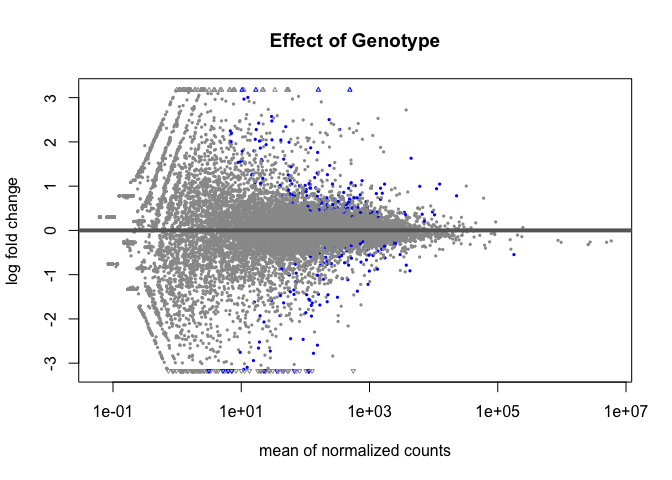
\includegraphics{figures-noura/ma-plot-1.png}

\begin{Shaded}
\begin{Highlighting}[]
\CommentTok{#x-axis is showing gene abundance , the more the count, the more to the right the dot will be }
\end{Highlighting}
\end{Shaded}

\begin{Shaded}
\begin{Highlighting}[]
\KeywordTok{library}\NormalTok{(pheatmap)}
\NormalTok{ntd <-}\StringTok{ }\KeywordTok{normTransform}\NormalTok{(dds)}
\NormalTok{selected.genes <-}\StringTok{ }\KeywordTok{order}\NormalTok{(dds.genotype}\OperatorTok{$}\NormalTok{padj)[}\DecValTok{1}\OperatorTok{:}\DecValTok{200}\NormalTok{] }\CommentTok{# pick the 50 most significantly changed genes (up vs down)}
\NormalTok{df <-}\StringTok{ }\KeywordTok{data.frame}\NormalTok{(}\KeywordTok{colData}\NormalTok{(dds)}\OperatorTok{$}\NormalTok{Genotype)}
\KeywordTok{rownames}\NormalTok{(df) <-}\StringTok{ }\KeywordTok{colnames}\NormalTok{(}\KeywordTok{assay}\NormalTok{(ntd)[selected.genes,])}
\NormalTok{df <-}\StringTok{ }\KeywordTok{rename}\NormalTok{(df, }\StringTok{'colData.dds..Genotype'}\NormalTok{=}\StringTok{'Genotype'}\NormalTok{)}
\KeywordTok{pheatmap}\NormalTok{(}\KeywordTok{assay}\NormalTok{(ntd)[selected.genes,],}
         \DataTypeTok{cluster_rows=}\NormalTok{T,}
         \DataTypeTok{show_rownames =}\NormalTok{ F,}
         \DataTypeTok{cluster_cols =}\NormalTok{ T,}
         \DataTypeTok{annotation_col=}\NormalTok{df,}
         \DataTypeTok{scale=}\StringTok{'row'}\NormalTok{,}
         \DataTypeTok{main=}\StringTok{"Significantly differentially expressed genes"}\NormalTok{)}
\end{Highlighting}
\end{Shaded}

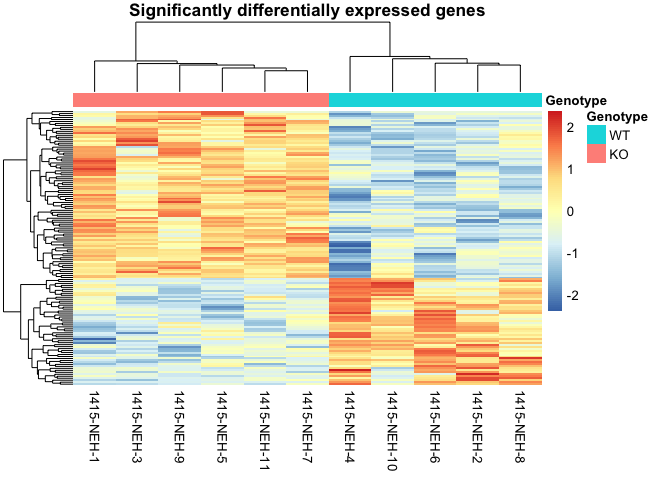
\includegraphics{figures-noura/heatmap-1.png}

\begin{Shaded}
\begin{Highlighting}[]
\NormalTok{selected.genes <-}\StringTok{ }\KeywordTok{order}\NormalTok{(dds.genotype}\OperatorTok{$}\NormalTok{padj)[}\DecValTok{1}\OperatorTok{:}\DecValTok{265}\NormalTok{]}
\KeywordTok{pheatmap}\NormalTok{(}\KeywordTok{assay}\NormalTok{(ntd)[selected.genes,],}
         \DataTypeTok{cluster_rows=}\NormalTok{T,}
         \DataTypeTok{show_rownames =}\NormalTok{ F,}
         \DataTypeTok{cluster_cols =}\NormalTok{ T,}
         \CommentTok{#annotation_col=df,}
         \DataTypeTok{scale=}\StringTok{'none'}\NormalTok{, }\CommentTok{#row is each row is the gene with each row having the same average value, normalized. In scale none, each row is still a ngene but no longer with normalized expression, harder to see since genes have different expression levels }
         \DataTypeTok{main=}\StringTok{"Top 200 Genotype modified genes"}\NormalTok{)}
\end{Highlighting}
\end{Shaded}

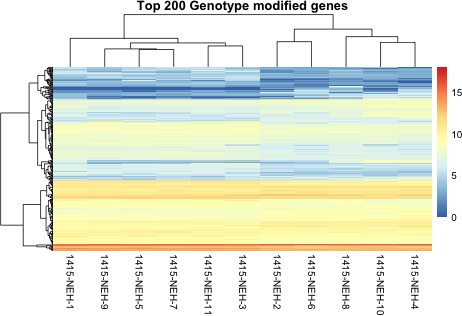
\includegraphics{figures-noura/heatmap-2.png}

\begin{Shaded}
\begin{Highlighting}[]
\CommentTok{#from https://www.biostars.org/p/282295/}

\CommentTok{#par(mar=c(5,5,5,5), cex=1.0, cex.main=1.4, cex.axis=1.4, cex.lab=1.4)}

\NormalTok{topT <-}\StringTok{ }\KeywordTok{as.data.frame}\NormalTok{(dds.genotype)}
\KeywordTok{library}\NormalTok{(ggplot2)}
\KeywordTok{ggplot}\NormalTok{(topT,(}\KeywordTok{aes}\NormalTok{(}\DataTypeTok{y=}\OperatorTok{-}\KeywordTok{log10}\NormalTok{(padj),}
                \DataTypeTok{x=}\NormalTok{log2FoldChange,}
                \DataTypeTok{col=}\NormalTok{padj}\OperatorTok{>}\FloatTok{0.05}\NormalTok{))) }\OperatorTok{+}
\StringTok{  }\KeywordTok{geom_point}\NormalTok{() }\OperatorTok{+}
\StringTok{  }\KeywordTok{labs}\NormalTok{(}\DataTypeTok{y=}\KeywordTok{bquote}\NormalTok{(}\OperatorTok{~-}\NormalTok{log[}\DecValTok{10}\NormalTok{]}\OperatorTok{~}\NormalTok{Q}\OperatorTok{~}\NormalTok{value),}
       \DataTypeTok{x=}\KeywordTok{bquote}\NormalTok{(}\OperatorTok{~}\NormalTok{log[}\DecValTok{2}\NormalTok{]}\OperatorTok{~}\NormalTok{fold}\OperatorTok{~}\NormalTok{change),}
       \DataTypeTok{subtitle=}\StringTok{"Adipocyte Tsc1 Knockout Mammary Gland RNAseq"}\NormalTok{) }\OperatorTok{+}
\StringTok{    }\KeywordTok{geom_text}\NormalTok{(}\DataTypeTok{data=}\KeywordTok{subset}\NormalTok{(topT, }\KeywordTok{abs}\NormalTok{(log2FoldChange) }\OperatorTok{>}\StringTok{ }\DecValTok{2} \OperatorTok{|}\StringTok{ }\OperatorTok{-}\KeywordTok{log10}\NormalTok{(padj) }\OperatorTok{>}\StringTok{ }\FloatTok{2.5}\NormalTok{),}
            \KeywordTok{aes}\NormalTok{(log2FoldChange,}\OperatorTok{-}\KeywordTok{log10}\NormalTok{(padj),}\DataTypeTok{label=}\NormalTok{symbol),}
            \DataTypeTok{check_overlap =} \OtherTok{TRUE}\NormalTok{, }\DataTypeTok{nudge_x =} \FloatTok{0.5}\NormalTok{) }\OperatorTok{+}
\StringTok{  }\KeywordTok{theme_classic}\NormalTok{() }\OperatorTok{+}
\StringTok{  }\KeywordTok{theme}\NormalTok{(}\DataTypeTok{text=}\KeywordTok{element_text}\NormalTok{(}\DataTypeTok{size=}\DecValTok{18}\NormalTok{),}
        \DataTypeTok{legend.position=}\StringTok{"none"}\NormalTok{) }\OperatorTok{+}
\StringTok{  }\KeywordTok{scale_colour_grey}\NormalTok{() }\OperatorTok{+}
\StringTok{  }\KeywordTok{xlim}\NormalTok{(}\OperatorTok{-}\DecValTok{5}\NormalTok{,}\DecValTok{5}\NormalTok{)}
\end{Highlighting}
\end{Shaded}

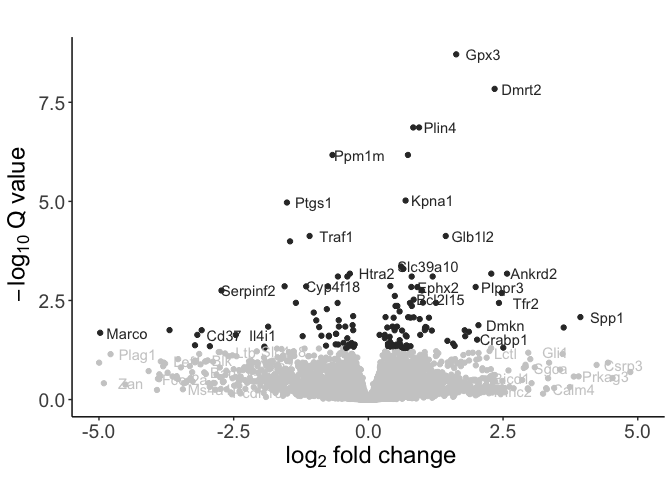
\includegraphics{figures-noura/volcano-plot-1.png}

\begin{Shaded}
\begin{Highlighting}[]
\CommentTok{#Adjusted P values (FDR Q values)}
\KeywordTok{with}\NormalTok{(topT, }\KeywordTok{plot}\NormalTok{(log2FoldChange, }\OperatorTok{-}\KeywordTok{log10}\NormalTok{(padj), }\DataTypeTok{pch=}\DecValTok{20}\NormalTok{, }\DataTypeTok{main=}\StringTok{"Volcano plot"}\NormalTok{, }\DataTypeTok{cex=}\FloatTok{1.0}\NormalTok{, }\DataTypeTok{xlab=}\KeywordTok{bquote}\NormalTok{(}\OperatorTok{~}\NormalTok{log[}\DecValTok{2}\NormalTok{]}\OperatorTok{~}\NormalTok{fold}\OperatorTok{~}\NormalTok{change), }\DataTypeTok{ylab=}\KeywordTok{bquote}\NormalTok{(}\OperatorTok{~-}\NormalTok{log[}\DecValTok{10}\NormalTok{]}\OperatorTok{~}\NormalTok{Q}\OperatorTok{~}\NormalTok{value)))}

\KeywordTok{with}\NormalTok{(}\KeywordTok{subset}\NormalTok{(topT, padj}\OperatorTok{<}\FloatTok{0.05} \OperatorTok{&}\StringTok{ }\KeywordTok{abs}\NormalTok{(log2FoldChange)}\OperatorTok{>}\DecValTok{2}\NormalTok{), }\KeywordTok{points}\NormalTok{(log2FoldChange, }\OperatorTok{-}\KeywordTok{log10}\NormalTok{(padj), }\DataTypeTok{pch=}\DecValTok{20}\NormalTok{, }\DataTypeTok{col=}\StringTok{"red"}\NormalTok{, }\DataTypeTok{cex=}\FloatTok{0.5}\NormalTok{))}

\CommentTok{#with(subset(topT, padj<0.05 & abs(log2FoldChange)>2), text(log2FoldChange, -log10(padj), labels=subset(rownames(topT), topT$padj<0.05 & abs(topT$log2FoldChange)>2), cex=0.8, pos=3))}

\CommentTok{#Add lines for absolute FC>2 and P-value cut-off at FDR Q<0.05}
\KeywordTok{abline}\NormalTok{(}\DataTypeTok{v=}\DecValTok{0}\NormalTok{, }\DataTypeTok{col=}\StringTok{"black"}\NormalTok{, }\DataTypeTok{lty=}\DecValTok{3}\NormalTok{, }\DataTypeTok{lwd=}\FloatTok{1.0}\NormalTok{)}
\KeywordTok{abline}\NormalTok{(}\DataTypeTok{v=}\OperatorTok{-}\DecValTok{2}\NormalTok{, }\DataTypeTok{col=}\StringTok{"black"}\NormalTok{, }\DataTypeTok{lty=}\DecValTok{4}\NormalTok{, }\DataTypeTok{lwd=}\FloatTok{2.0}\NormalTok{)}
\KeywordTok{abline}\NormalTok{(}\DataTypeTok{v=}\DecValTok{2}\NormalTok{, }\DataTypeTok{col=}\StringTok{"black"}\NormalTok{, }\DataTypeTok{lty=}\DecValTok{4}\NormalTok{, }\DataTypeTok{lwd=}\FloatTok{2.0}\NormalTok{)}
\KeywordTok{abline}\NormalTok{(}\DataTypeTok{h=}\OperatorTok{-}\KeywordTok{log10}\NormalTok{(}\KeywordTok{max}\NormalTok{(topT}\OperatorTok{$}\NormalTok{pvalue[topT}\OperatorTok{$}\NormalTok{padj}\OperatorTok{<}\FloatTok{0.05}\NormalTok{], }\DataTypeTok{na.rm=}\OtherTok{TRUE}\NormalTok{)), }\DataTypeTok{col=}\StringTok{"black"}\NormalTok{, }\DataTypeTok{lty=}\DecValTok{4}\NormalTok{, }\DataTypeTok{lwd=}\FloatTok{2.0}\NormalTok{)}
\end{Highlighting}
\end{Shaded}

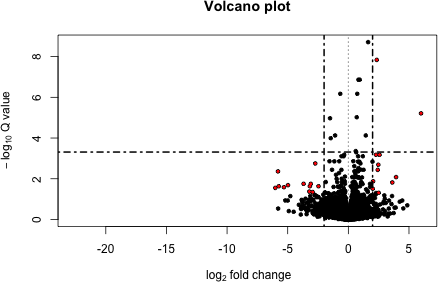
\includegraphics{figures-noura/volcano-plot-2.png}

\hypertarget{principal-components-analysis}{%
\section{Principal Components
Analysis}\label{principal-components-analysis}}

\begin{Shaded}
\begin{Highlighting}[]
\NormalTok{vsd <-}\StringTok{ }\KeywordTok{vst}\NormalTok{(dds, }\DataTypeTok{blind=}\OtherTok{FALSE}\NormalTok{)}
\KeywordTok{plotPCA}\NormalTok{(vsd, }\DataTypeTok{intgroup=}\KeywordTok{c}\NormalTok{(}\StringTok{"Genotype"}\NormalTok{)) }\CommentTok{#overall seeing how similar samples are to each other, across sample variance, this is not due to genotype since the genotypes are not clustered alone in two separate clusters}
\end{Highlighting}
\end{Shaded}

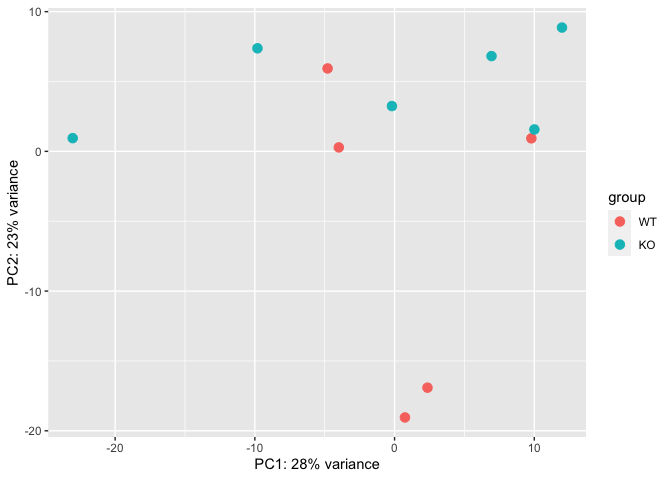
\includegraphics{figures-noura/pca-1.png}

\begin{Shaded}
\begin{Highlighting}[]
\NormalTok{output.file <-}\StringTok{ 'Noura DESeq2 Results - Genotype.csv'}
\NormalTok{output.counts <-}\StringTok{ 'Noura DESeq2 Normalized Counts.csv'}
\NormalTok{output.design <-}\StringTok{ 'Noura Design Table.csv'}

\KeywordTok{write.csv}\NormalTok{(}\KeywordTok{as.data.frame}\NormalTok{(dds.genotype), }\DataTypeTok{file=}\NormalTok{output.file)}
\KeywordTok{write.csv}\NormalTok{(}\KeywordTok{counts}\NormalTok{(dds, }\DataTypeTok{normalized=}\NormalTok{T), }\DataTypeTok{file=}\NormalTok{output.counts)}
\KeywordTok{write.csv}\NormalTok{(coldata, }\DataTypeTok{file=}\NormalTok{output.design)}
\end{Highlighting}
\end{Shaded}

\hypertarget{session-information}{%
\section{Session Information}\label{session-information}}

\begin{Shaded}
\begin{Highlighting}[]
\KeywordTok{sessionInfo}\NormalTok{()}
\end{Highlighting}
\end{Shaded}

\begin{verbatim}
## R version 4.0.2 (2020-06-22)
## Platform: x86_64-apple-darwin17.0 (64-bit)
## Running under: macOS  10.16
## 
## Matrix products: default
## BLAS:   /Library/Frameworks/R.framework/Versions/4.0/Resources/lib/libRblas.dylib
## LAPACK: /Library/Frameworks/R.framework/Versions/4.0/Resources/lib/libRlapack.dylib
## 
## locale:
## [1] en_US.UTF-8/en_US.UTF-8/en_US.UTF-8/C/en_US.UTF-8/en_US.UTF-8
## 
## attached base packages:
## [1] parallel  stats4    stats     graphics  grDevices utils     datasets 
## [8] methods   base     
## 
## other attached packages:
##  [1] ggplot2_3.3.3               pheatmap_1.0.12            
##  [3] org.Mm.eg.db_3.12.0         AnnotationDbi_1.52.0       
##  [5] DESeq2_1.30.1               SummarizedExperiment_1.20.0
##  [7] Biobase_2.50.0              MatrixGenerics_1.2.1       
##  [9] matrixStats_0.58.0          GenomicRanges_1.42.0       
## [11] GenomeInfoDb_1.26.4         IRanges_2.24.1             
## [13] S4Vectors_0.28.1            BiocGenerics_0.36.0        
## [15] tximeta_1.8.4               tximport_1.18.0            
## [17] dplyr_1.0.5                 tidyr_1.1.3                
## [19] knitr_1.31                 
## 
## loaded via a namespace (and not attached):
##  [1] colorspace_2.0-0              ellipsis_0.3.1               
##  [3] XVector_0.30.0                farver_2.1.0                 
##  [5] bit64_4.0.5                   interactiveDisplayBase_1.28.0
##  [7] fansi_0.4.2                   xml2_1.3.2                   
##  [9] splines_4.0.2                 cachem_1.0.4                 
## [11] geneplotter_1.68.0            jsonlite_1.7.2               
## [13] Rsamtools_2.6.0               annotate_1.68.0              
## [15] dbplyr_2.1.0                  shiny_1.6.0                  
## [17] BiocManager_1.30.12           readr_1.4.0                  
## [19] compiler_4.0.2                httr_1.4.2                   
## [21] assertthat_0.2.1              Matrix_1.3-2                 
## [23] fastmap_1.1.0                 lazyeval_0.2.2               
## [25] later_1.1.0.1                 htmltools_0.5.1.1            
## [27] prettyunits_1.1.1             tools_4.0.2                  
## [29] gtable_0.3.0                  glue_1.4.2                   
## [31] GenomeInfoDbData_1.2.4        rappdirs_0.3.3               
## [33] Rcpp_1.0.6                    vctrs_0.3.7                  
## [35] Biostrings_2.58.0             rtracklayer_1.50.0           
## [37] xfun_0.22                     stringr_1.4.0                
## [39] mime_0.10                     lifecycle_1.0.0              
## [41] ensembldb_2.14.0              XML_3.99-0.6                 
## [43] AnnotationHub_2.22.0          zlibbioc_1.36.0              
## [45] scales_1.1.1                  hms_1.0.0                    
## [47] promises_1.2.0.1              ProtGenerics_1.22.0          
## [49] AnnotationFilter_1.14.0       RColorBrewer_1.1-2           
## [51] yaml_2.2.1                    curl_4.3                     
## [53] memoise_2.0.0                 biomaRt_2.46.3               
## [55] stringi_1.5.3                 RSQLite_2.2.5                
## [57] BiocVersion_3.12.0            highr_0.8                    
## [59] genefilter_1.72.1             GenomicFeatures_1.42.2       
## [61] BiocParallel_1.24.1           rlang_0.4.10                 
## [63] pkgconfig_2.0.3               bitops_1.0-6                 
## [65] evaluate_0.14                 lattice_0.20-41              
## [67] purrr_0.3.4                   labeling_0.4.2               
## [69] GenomicAlignments_1.26.0      bit_4.0.4                    
## [71] tidyselect_1.1.0              magrittr_2.0.1               
## [73] R6_2.5.0                      magick_2.7.1                 
## [75] generics_0.1.0                DelayedArray_0.16.3          
## [77] DBI_1.1.1                     pillar_1.5.1                 
## [79] withr_2.4.1                   survival_3.2-10              
## [81] RCurl_1.98-1.3                tibble_3.1.0                 
## [83] crayon_1.4.1                  utf8_1.2.1                   
## [85] BiocFileCache_1.14.0          rmarkdown_2.7                
## [87] progress_1.2.2                locfit_1.5-9.4               
## [89] grid_4.0.2                    blob_1.2.1                   
## [91] digest_0.6.27                 xtable_1.8-4                 
## [93] httpuv_1.5.5                  openssl_1.4.3                
## [95] munsell_0.5.0                 askpass_1.1
\end{verbatim}

\end{document}
